\documentclass[a4paper, 12pt]{article}

\usepackage{fancyhdr}
\pagestyle{fancy}
\lhead{PROJET : Forteresse}
\lfoot{Info Sup}
\rfoot{EPITA 2016}
\renewcommand{\footrulewidth}{0.3mm}

\usepackage[french]{babel}
\usepackage{listings}
\usepackage[T1]{fontenc}
\usepackage{eurosym}
\usepackage{setspace}
\usepackage{caption}

\usepackage[utf8]{inputenc}
\usepackage{graphicx}

\renewcommand{\baselinestretch}{1.5}
\begin{document}
\begin{titlepage}
  \begin{sffamily}
  \begin{center}

    % Upper part of the page. The '~' is needed because \\
    % only works if a paragraph has started.

    \textsc{\Huge Rapport soutenance 1}\\[3cm]

    \textsc{\LARGE Projet:}\\[1.5cm]

    % Title
	\centerline{
\includegraphics{coollogo_com-19602433.png}}
	\vfill{
	\centerline{
\includegraphics[scale=0.4]{crossed-swords-clip-art-48219.jpg}}}

    % Author and supervisor
    \begin{minipage}{0.4\textwidth}
      \begin{flushleft} \large	
      
      \end{flushleft}
    \end{minipage}
	\begin{flushleft}\vfill
      {
       \textsc{Chatelus} Florian - \emph{chatel\_f} \\
       \textsc{Henric} Arnaud - \emph{henric\_a}\\
       \textsc{Sarkar} Riday - \emph{sarkar\_r}\\
       \textsc{Ezzahoui} Yassine - \emph{ezzaho\_y} }
    \end{flushleft}	
  \end{center}
  \end{sffamily}
\end{titlepage}

\begin{spacing}{1.0}
	\tableofcontents
\end{spacing}

\newpage
\section{Introduction}
Dans le cadre de de notre première année à l'EPITA, nous devons réaliser un projet informatique de fin d'année qui doit montrer l'application de nos connaissances dans le domaine de la programmation.
	Le sujet étant libre, nous avons décidé de réaliser un jeu vidéo nommé Forteresse.
	Le présent document est  le rapport de la première soutenance qui retrace l'avancement de notre projet en cours de développement depuis la validation du cahier des charges jusqu'à la première soutenance. Ainsi, à travers ce rapport, nous allons établir un bilan des tâches qui ont été réalisées par chacun des membres du groupe. Nous allons aussi établir un bilan  des tâches qui restent à  réaliser pour  la prochaine soutenance.

\newpage

\section{Présentation}
	\subsection{Les membres du groupe}
	\parindent=0cm\textbf{Florian \textsc{Chatelus}}
	\smallbreak
	\par \parindent=0.5cm Commence enfin l'une des raisons pour laquelle j'ai choisi l'EPITA, le projet! A mon arrivé a l'EPITA la programmation ne m'était pas totalement inconnue puisque j'ai eu la chance de pouvoir choisir la spécialisation ISN en Terminale. Nous avions réussi avec mon groupe a recréer le célèbre PONG. Bien que mon projet d'ISN ai été très basique, je pense qu'il me servira au moins dans les démarches de réalisation du projet. J'ai donc une petite expérience en ce qui concerne le travail de groupe, que j'espère arriver a mettre a profit pour notre projet de cette année. Malgré tout, ce projet sera un réel challenge pour moi, puisqu'il nous obligera a faire appel a de nombreuse compétence que nous ne disposons pas encore. Ce sera donc un formidable exercice, qui demandera une certaine rigueur dans le travail certes, mais qui me permettra de progresser rapidement.\\
	
	\parindent=0cm\textbf{Arnaud \textsc{Henric}}
	\smallbreak
	Le projet de première année, enfin ! Nous avons déjà eu des TPs de programmation mais le projet permettra de nous tester d’avantage. En groupe, nous allons réaliser un devoir que nous avons nous-mêmes choisi, un jeu-vidéo. J’ai déjà réaliser certains projets en ISN au lycée (le triangle de Sierpinski, le jeu de la vie ou encore un code barre) mais jamais de projet comme celui-ci, sur un semestre entier et en groupe. Néanmoins ISN m’a donné un peu d'expérience et je suis prêt à créer ce jeu vidéo.\\
\newpage	
	\parindent=0cm\textbf{Riday \textsc{Sarkar}}
	\smallbreak
 Avant d’arriver à EPITA,  j'ai jamais touché à une ligne de code à part cliquer de temps en temps sur des icônes avec Algobox en cours de maths (au passage c'était très bien pour découvrir  le monde merveilleux de l’algorithmique). Je suis conscient que réaliser les tâches qu’on m’a données ne sera pas facile. Cela étant dit, je sais que ce projet est un plus pour nous et qu’on va apprendre beaucoup de choses à travers la réalisation de ce projet. Donc je vais jouer le jeu et faire un maximum de choses pour le projet et essayer d’apprendre un maximum de choses à travers la réalisation de ce projet.\\

	\parindent=0cm\textbf{Yassine \textsc{Ezzahoui}}
	\smallbreak
	Nous abordons  le projet de première année avec ambition et envie , nombreux seront les défis à relever. Pour ma part avant cette année je n’avais aucune notion en programmation, ce projet me permettra donc d’apprendre différents langage de programmation,  de connaître tous les paramètres qui régissent un travail de groupe de cette ampleur. Ainsi ce  projet est pour moi  un atout pour l’apprentissage de tout les aspects que peut m'offrir la programmation.\\
	
	Nous tenons à vous informer qu'un membre du groupe, Yassine \textsc{Ezzahoui}, a quitt\'e l'EPITA.   

	\parindent=0.5cm 
	\subsection{Les origines du projet}
Nous avons choisi de réaliser un jeu plutôt qu’un logiciel car nous avons deux membres dans le groupe qui ont déjà réalisé un jeu en Terminale dans le cadre d’un projet en groupe. Même si le projet achevé en ISN par ces deux derniers n’est pas comparable avec ce qui nous attend ce semestre en INFO SUP, ce sera toujours une aide non-négligeable.
\par Une fois que la nature du projet était choisi, nous avons réfléchi longuement sur le type de jeu que nous allons réaliser. Notre expérience en tant que joueur nous donnait un large choix parmi les types de jeu possibles comme un RPG (Role Playing Game), RTS (Real Time Strategy) ou encore un Tower Defense . 

	\subsection{Le jeu}
		\subsubsection{Présentation}
		\par Notre jeu sera basé sur le principe du \textit{tower defense}. Qu'est-ce que 			cela signifie? Un \textit{tower defense}, est un jeu qui comme son nom l'indique 			aura comme objectif de défendre un point donné. Le but du jeu sera donc de défendre 		un cristal qui alimente la porte de l'endroit que nous souhaitons protéger.  
		\subsubsection{Déroulement d'une partie}
		Une partie se déroulera en deux phases qui se répéteront, a chaque vague d'ennemis.\\
		\centerline{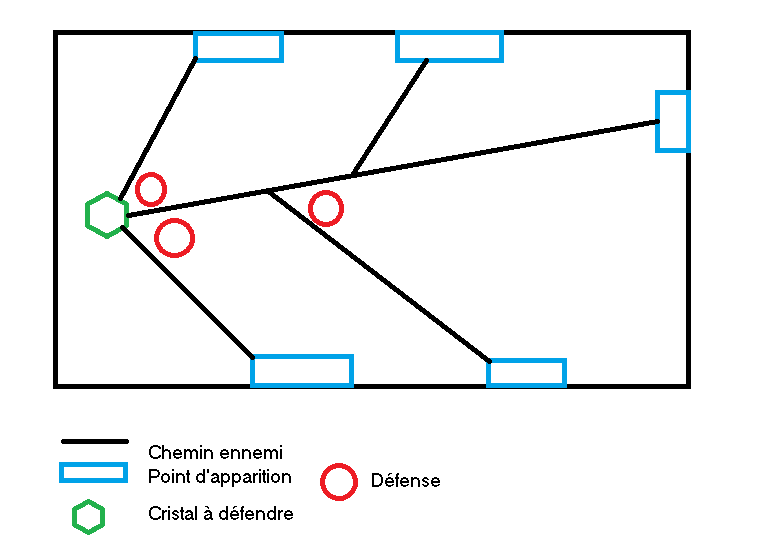
\includegraphics[scale=0.55]{Plan.png}}
		\par La première est la phase que nous appellerons \textit{phase de préparation}, elle consiste à préparer ses défenses, en les positionnant de façon stratégique, les améliorant ou en les réparant. Cette phase sera d'une importance capital pour assurer une victoire lors de la phase suivante. Une fois que vous serez fin prêt pour le combat, il vous suffira d'appuyer sur prêt et la deuxième phase commencera une fois tout les joueurs prêt.
		\par Nous arrivons donc en deuxième phase, la \textit{phase de combat}, qui va déclencher l'action. Des créatures vont apparaitre à des points précis de la carte et vont converger vers le ou les cristaux. Le joueur pourra donc durant cette phase attaquer les monstres et tenter de les détruire et/ou continuer à poser, améliorer et réparer ses constructions mais avec des malus d'incantation.
		\bigbreak
		\begin{figure}[!ht]
			\centerline{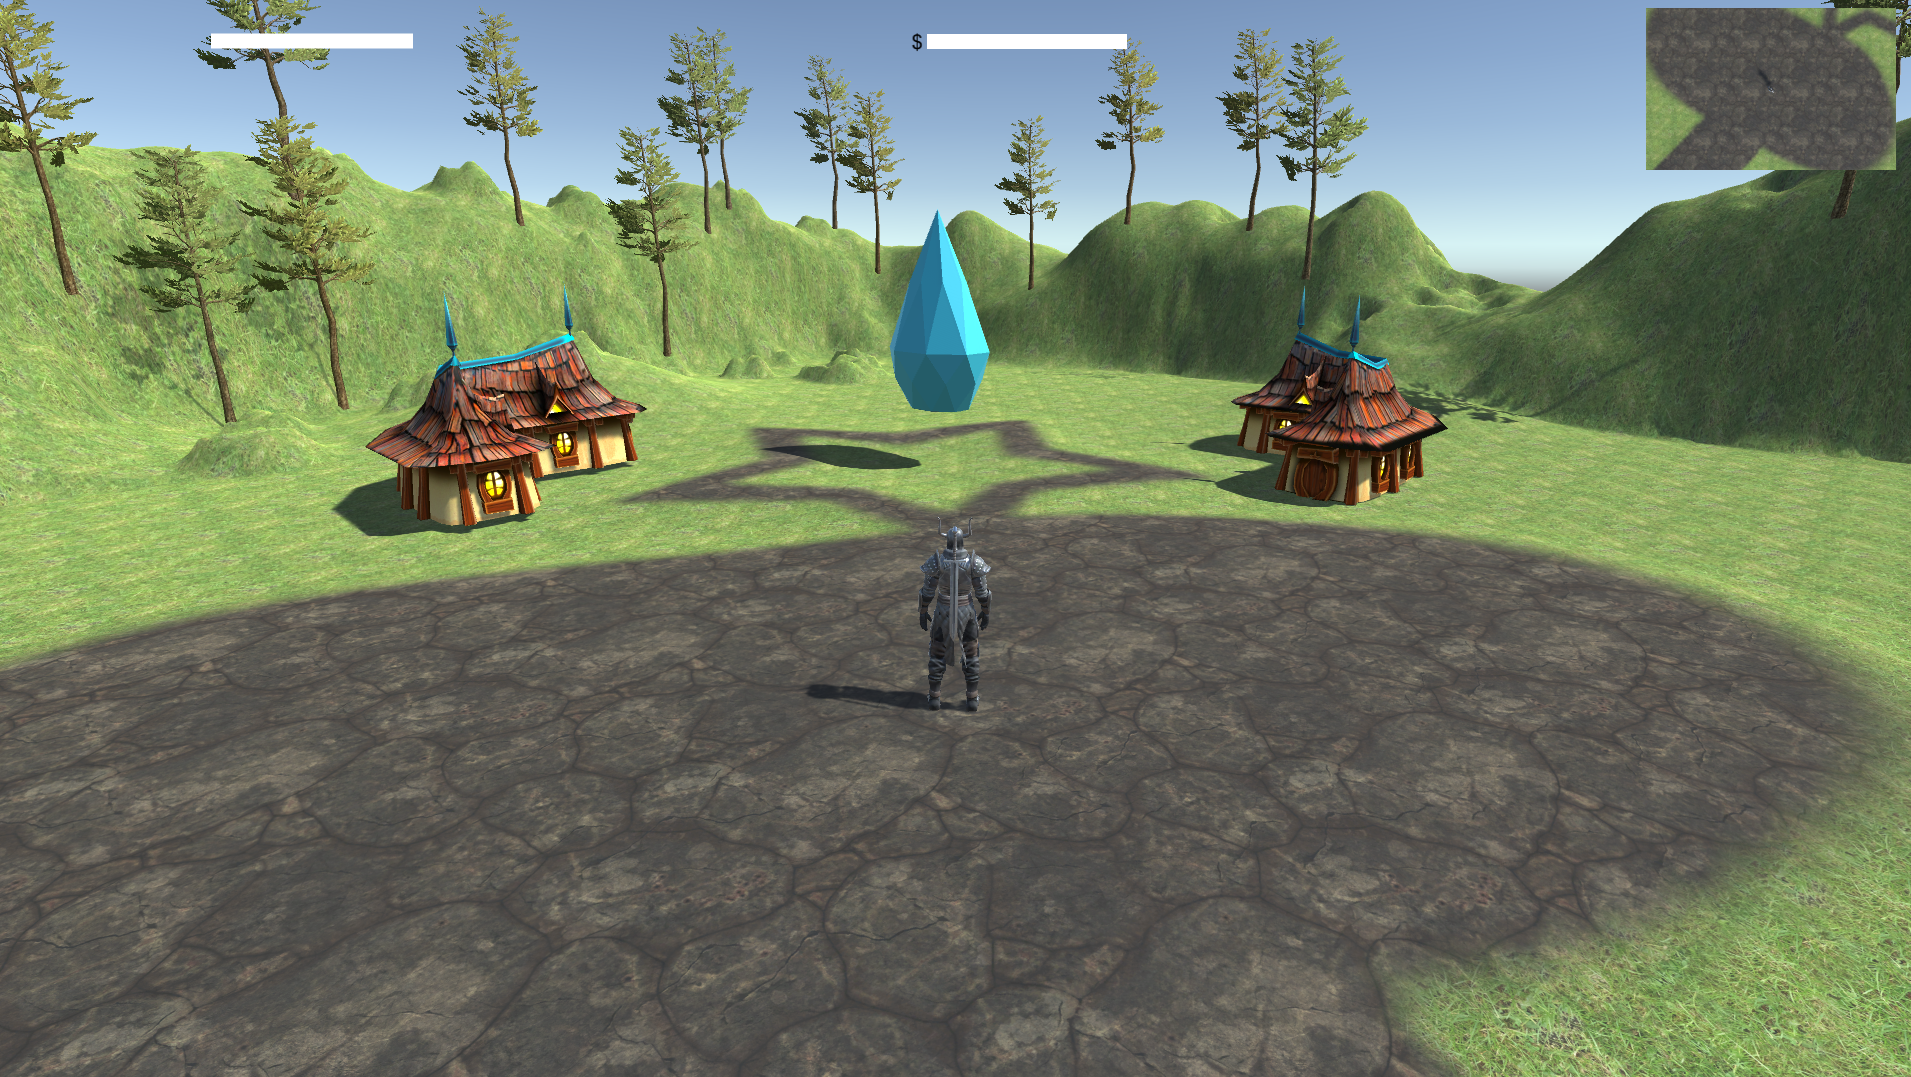
\includegraphics[scale=0.3]{cristalprojet.png}}
			\caption*{Image du cristal à protéger}
		\end{figure}
		\par Tous les certains nombre de cycle, au terme de ces deux phases, un monstre plus imposant apparaitra, et le joueur devra s'en défaire afin de remporter la manque et d'obtenir des objets.
		\subsubsection{Multijoueur}
		Le mode multijoueur consistera en un mode CO-OP. Vous devrez \^etre capable de jouer en \'equipe afin d'affronter vos adversaires. Pour cela, vous commencerez la partie c\^ote \'a c\^ote. Vous ne pouvez combattre seulement des IA. Le mode multijoueur consiste en un mode en \'equipe et non pas en 1vs1 contre un ami.
		\par Chaque joueur pourra int\'eragir avec l'environnement. Leurs constructions et leurs objectifs sont communs tandis que toutes leurs caract\'eristiques telles que leur monnaie et leur vie sont s\'epar\'ees.
		\subsubsection{L'interface}
		L’interface permettra au joueur d'être renseignée à tout moment sur : 
		\begin{itemize}
		\item Le temps écoulé.
		\item Sa jauge de vie.
		\item L’arme dont il est en possession , ainsi que les  munitions dont il dispose.
		\item L’argent qu’il possède pour acheter de nouvelles tours ou armes.
		\end{itemize}
		\subsubsection{L'arsenal de défense}
		Nous utiliserons donc différents types d’armes de type médiéval fantastique.
Les armes seront donc accessible en la ramassant sur un bosse ou bien  suite à un achat du joueur, elles pourront être améliorer, durant la partie. On distinguera plusieurs types d’armes tel que:
	\begin{itemize}
	\item Les épées.
	\item Les arcs.
	\item Les bâtons.
	\end{itemize}
Les défenses fixes seront achetable grâce a l’argent gagné durant la partie. Les défenses seront comme les armes améliorables. Ces dernières seront autonomes et feront partie de l’IA. On pourra y trouver:
	\begin{itemize}
	\item Des tourelles.
	\item Des pièges.
	\item Des auras.
	\end{itemize}
\newpage
\section{Répartition des tâches}
Nous avions au départ attribué deux personnes a chaque tâche, afin de pouvoir nous entre aider. cela nous a servit puisqu'un membre du groupe nous a quitté, toute les tâches ont donc gardé au moins une personne attribué. Mais il s'est avéré plus efficace de se spécialiser dans des domaines précis plutôt que de toucher a beaucoup de domaine et de travailler a plusieurs sur ceux-ci.\\
Le tableau ci dessous montre quelles ont été les tâches effectué et par qui.
\bigbreak
\bigbreak
	\begin{tabular}{|c||c|c|c|c|c|}
		\hline
		& Florian & Riday & Yassine & Arnaud \\
		\hline
		Site & & & $\times$ & $\times$\\
		\hline
		3D & & $\times$ & &\\
		\hline
		2D & & $\times$ & & \\
		\hline
		IA & $\times$ & & & \\
		\hline
		Multijoueur &  & &  &\\
		\hline
		Réseau & & $\times$ & & \\
		\hline
		Menu & & & & $\times$\\
		\hline
		Gameplay & $\times$ & & &\\
		\hline
		Animation & $\times$ & $\times$ & & \\		
		\hline
		Audio & & & & $\times$\\
		\hline
		\LaTeX & $\times$ & $\times$ & $\times$ & $\times$\\
		\hline
	\end{tabular}
	\newpage
\newpage
\section{Avancement du projet}
	\subsection{Le graphisme}
		\subsubsection{La carte}
		Nous nous sommes mis d’accord pour une carte plutôt fermée. Nous avons donc décidé d’entourer le terrain par des chaînes de montagnes. Comme le jeu se déroule à l’époque médiévale, nous avons décidé d’avoir un terrain plutôt vert avec des arbres et des maisons médiévales. Nous avons des maisons de l’époque médiévale sur le terrain mais pas encore des villages. Nous savons très bien que les villages n’interviennent pas dans le jeu mais ils permettent d’avoir un environnement du jeu riche en détails. 
\par Le apparition des ennemis se fait derrière les chaînes de montagnes. Ensuite, ils se dirigent vers le cristal en suivant un chemin visible qu’on a tracé. Le joueur voit les différents chemins qui vont être empruntés par les ennemis et ensuite il place des tours tout au long de ces chemins qui vont tuer les ennemis et ainsi empêcher l’arrivée des ennemis jusqu’au cristal.

		\subsubsection{La 3D}
		Yassine devait modéliser les personnages avec Blender mais après qu’il ait quitté EPITA et rendu son travail sur le site, nous avons décidé de ne pas passer moins de temps sur la création des personnages et des élément du jeu.  Pour le moment, nous travaillons avec deux modèles de personnages importés de l’asset store mais c’est provisoire. Nous comptons avoir des monstres qui vont constituer les ennemis et plusieurs modèles de personnages. Ainsi le joueur a la possibilité de choisir le personnage qui lui convient.  
\par Le cristal est l’élément majeur de notre jeu car le jeu consiste à défendre ce cristal. Nous avons décidé d’importer un diamant depuis Blender, le logiciel 3D qu’on utilise, et de le transformer en forme de cristal avec Unity, le moteur de jeu. Nous l’avons ensuite ajouté une texture pour le visuel et une force pour qu’il puisse flotter.

		\subsubsection{La 2D}
Nous avons une minimap qui permet d’avoir une vue d’ensemble et qui suit le joueur en permanence. Pour cela, nous sommes passés par un script C\#.  Pour l’instant, nous n’avons pas pu faire en sorte de distinguer le joueur sur la minimap des autres éléments qui l’entourent.
\par Nous avons mis en place la barre de vie et la barre représentant l'argent dont le joueur dispose car chaque construction de tour coûtera de l’argent au joueur. Elles ne sont pas encore fonctionnelles car nous n’avons pas encore défini le système de vie et d'argent.
\subsubsection*{Ce qui est à faire pour la prochaine soutenance}
\begin{itemize}
\item Nous avons certes décidé de ne pas changer la carte à chaque niveau mais au menu principal, le joueur aura le choix entre plusieurs cartes avec des décors différents. Nous comptons faire au moins une seconde carte.
\item Faire en sorte que l'on puisse distinguer le joueur parmi les différents éléments de la carte qui l’entourent.
\item Avoir plusieurs modèles de personnages et d'ennemis
\item Rendre fonctionnelles les barres de vie et d’argent

\end{itemize}

\newpage

	\subsection{Le réseau}
Nous avons mis en place un réseau en mode \emph{host} en utilisant le network manager d’Unity. Un joueur se porte comme serveur et les autres joueurs sont donc des clients.\\


\begin{figure}[!ht]
	\centerline{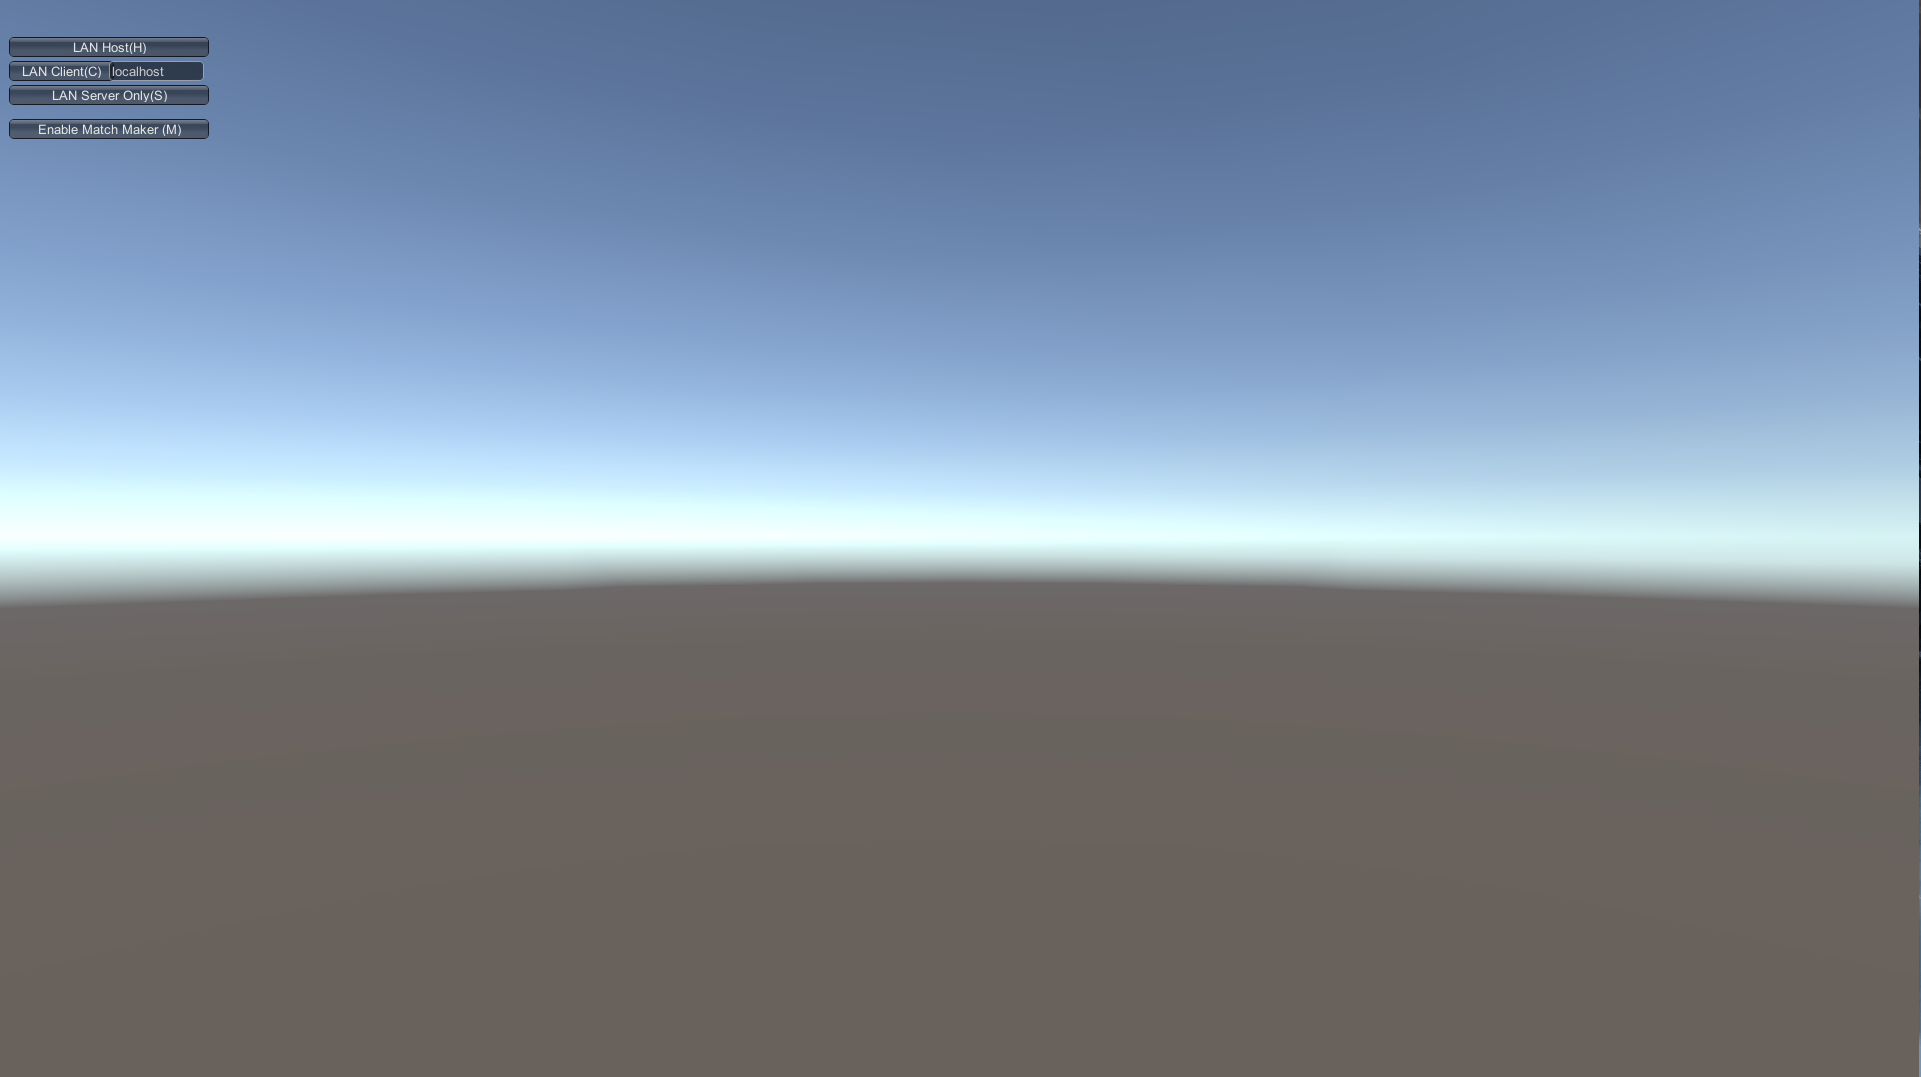
\includegraphics[scale=0.3]{Menureseauprojet.png}}
	\caption*{Image du menu pour jouer en réseau}
\end{figure}

\subsubsection*{Ce qui est à faire pour la prochaine soutenance}

\par Certes nous avons mis en place le réseau, mais pour l’instant, le joueur qui se comporte comme serveur peut commencer une partie sans qu’il y ait d’autres joueurs présents en ligne. Donc il faut recoder le network manager  pour que joueur qui va se comporter comme serveur ne puisse pas lancer la partie tant qu’il n'y ait pas au moins un autre joueur en ligne.

\newpage
	\subsection{Multijoueur}
	Notre manque d'expériences dans le domaine de la création de jeu vidéo, nous a forcé \'a planifier l'avancement de notre projet sans de réels prévisions. C'est pour cela que le multijoueur n'a pas encore été débuté a l'heure actuelle. Il sera débuté lorsque le réseau sera pleinement opérationnel. 
	
	\subsection{L'intelligence artificiel}
	L'intelligence artificiel (IA) a été une de nos priorités lors pour cette première soutenance, car elle est un outil majeur du bon fonctionnement du jeu. A l'heure actuelle l'IA est très basique. Elle permet simplement aux ennemis de se déplacer d'un point A \'a  un point B, en suivant un chemin défini au préalable.
	
\subsubsection*{Ce qui est à faire pour la prochaine soutenance}	
	
	\par La prochaine étape sera de lui permettre de converger vers un objet lorsque celui-ci sera \'a sa portée et bien évidemment de l'attaquer, afin d'avoir une IA fonctionnelle, permettant le déroulement d'une partie.

	\subsection{Le menu}
	

	\par Nous avons réalisé le menu principal, le menu d’options ainsi que le menu de pause dans le jeu. Le menu principal nous permet de lancer le jeu en solo, nous diriger vers le multijoueur mais également de nous envoyer vers le sous-menu pour les options. Enfin il permet évidemment de quitter le jeu avec un message de confirmation.
Ensuite, le sous-menu qui gère les options du jeu permet de modifier le volume du son dans le menu. Il permettra ensuite de gérer la luminosité et de donner d’autres indications.
\newpage
	\begin{figure}[!ht]
		\centerline{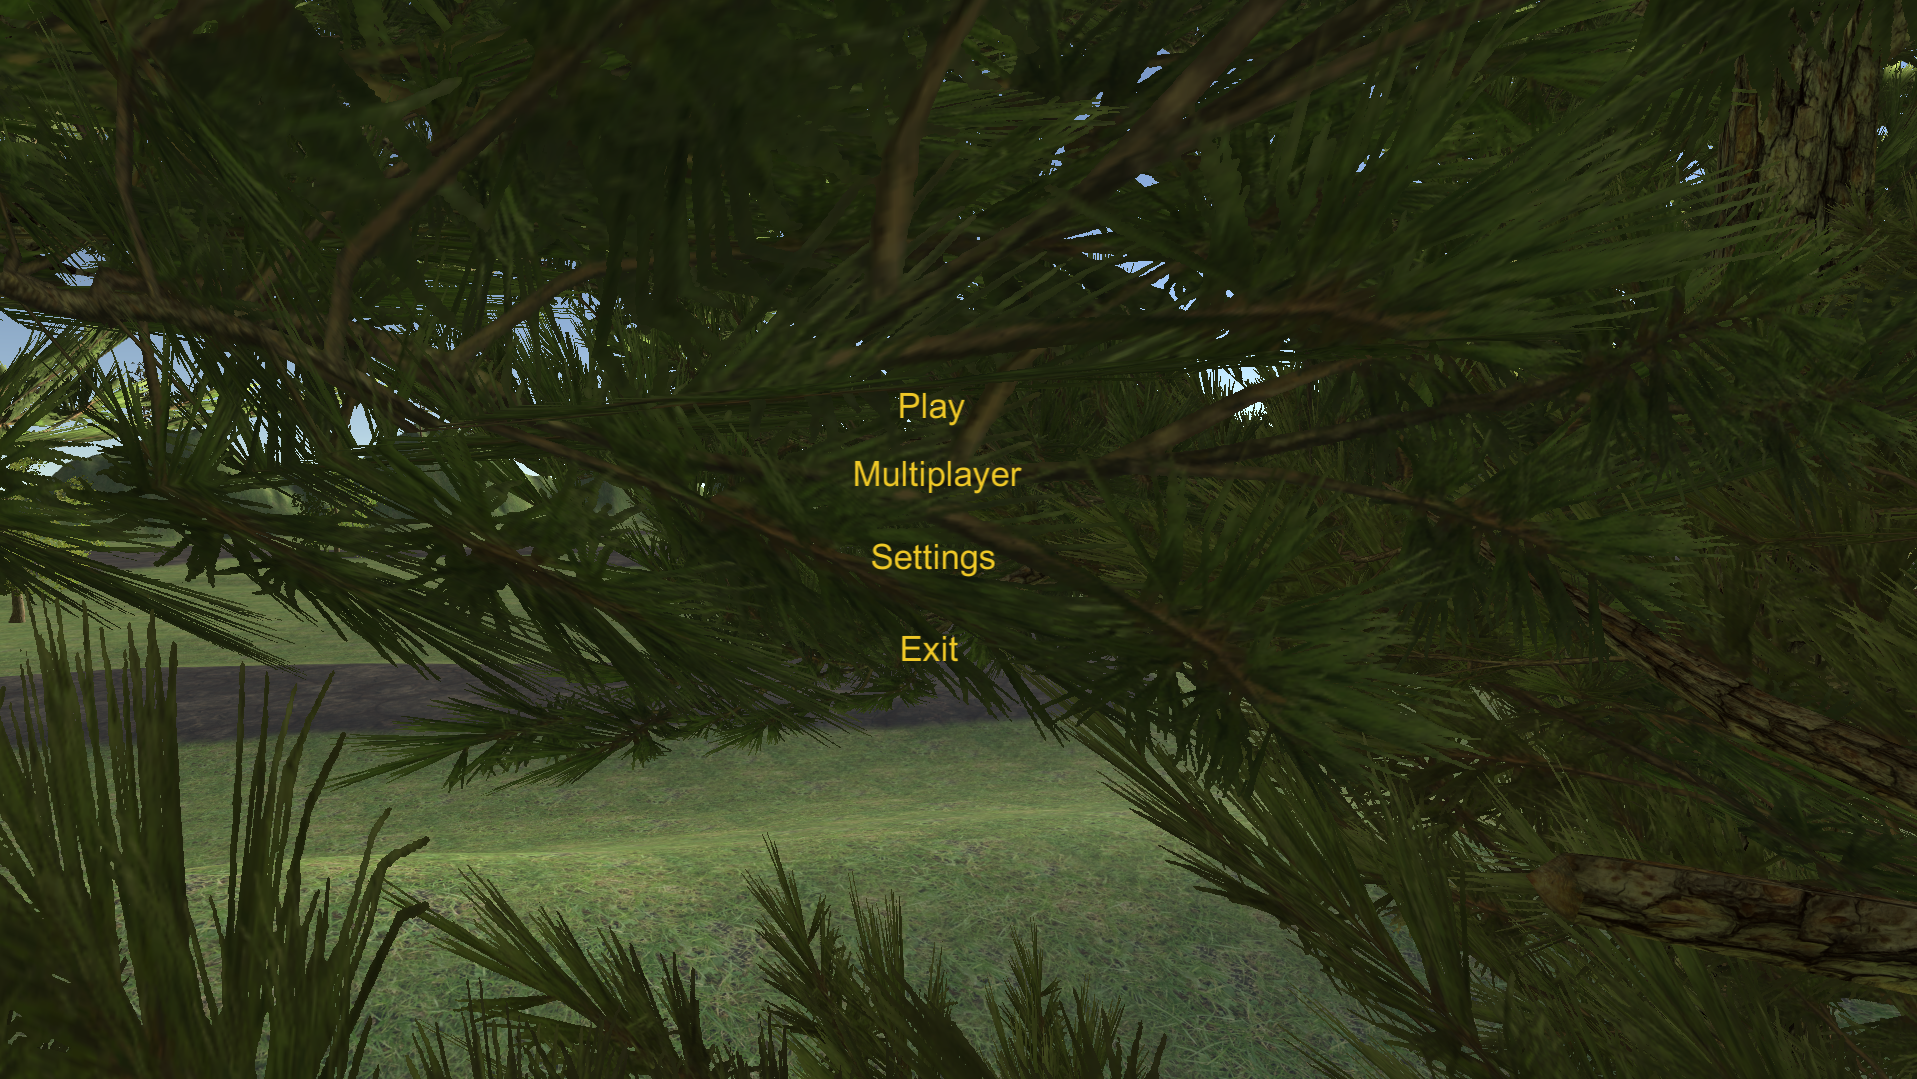
\includegraphics[scale=0.3]{Menuprojet.png}}
		\caption*{Image du menu principal}		
	\end{figure}
	\begin{figure}[!ht]
		\centerline{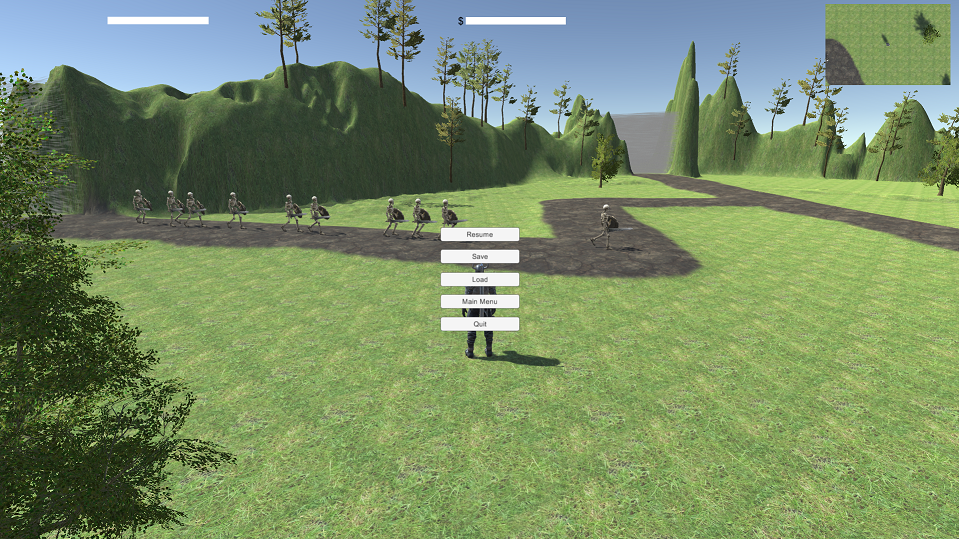
\includegraphics[scale=0.3]{Menupauseprojet.png}}
		\caption*{Image du menu pause}
	\end{figure}
	
	\par Enfin, nous avons également créer un menu-pause qui apparaît lorsqu’on appuie sur “echap” dans le jeu. Il arrête bien sûr le jeu (les mouvements des personnages et les attaques) lorsqu’il est actif. Dans le menu pause, on peut évidemment reprendre le jeu en cours au même moment, mais également relancer le niveau et revenir au menu principal. On pourra ensuite sauvegarder le jeu, pour le reprendre plus tard.

	\subsection{Le site}
	 Le site internet devait être réalisé avec Yassine. Avec son départ de l’EPITA, l’objectif était de réaliser un site qui fonctionne. 
	 
	\begin{figure}[!ht]
		\centerline{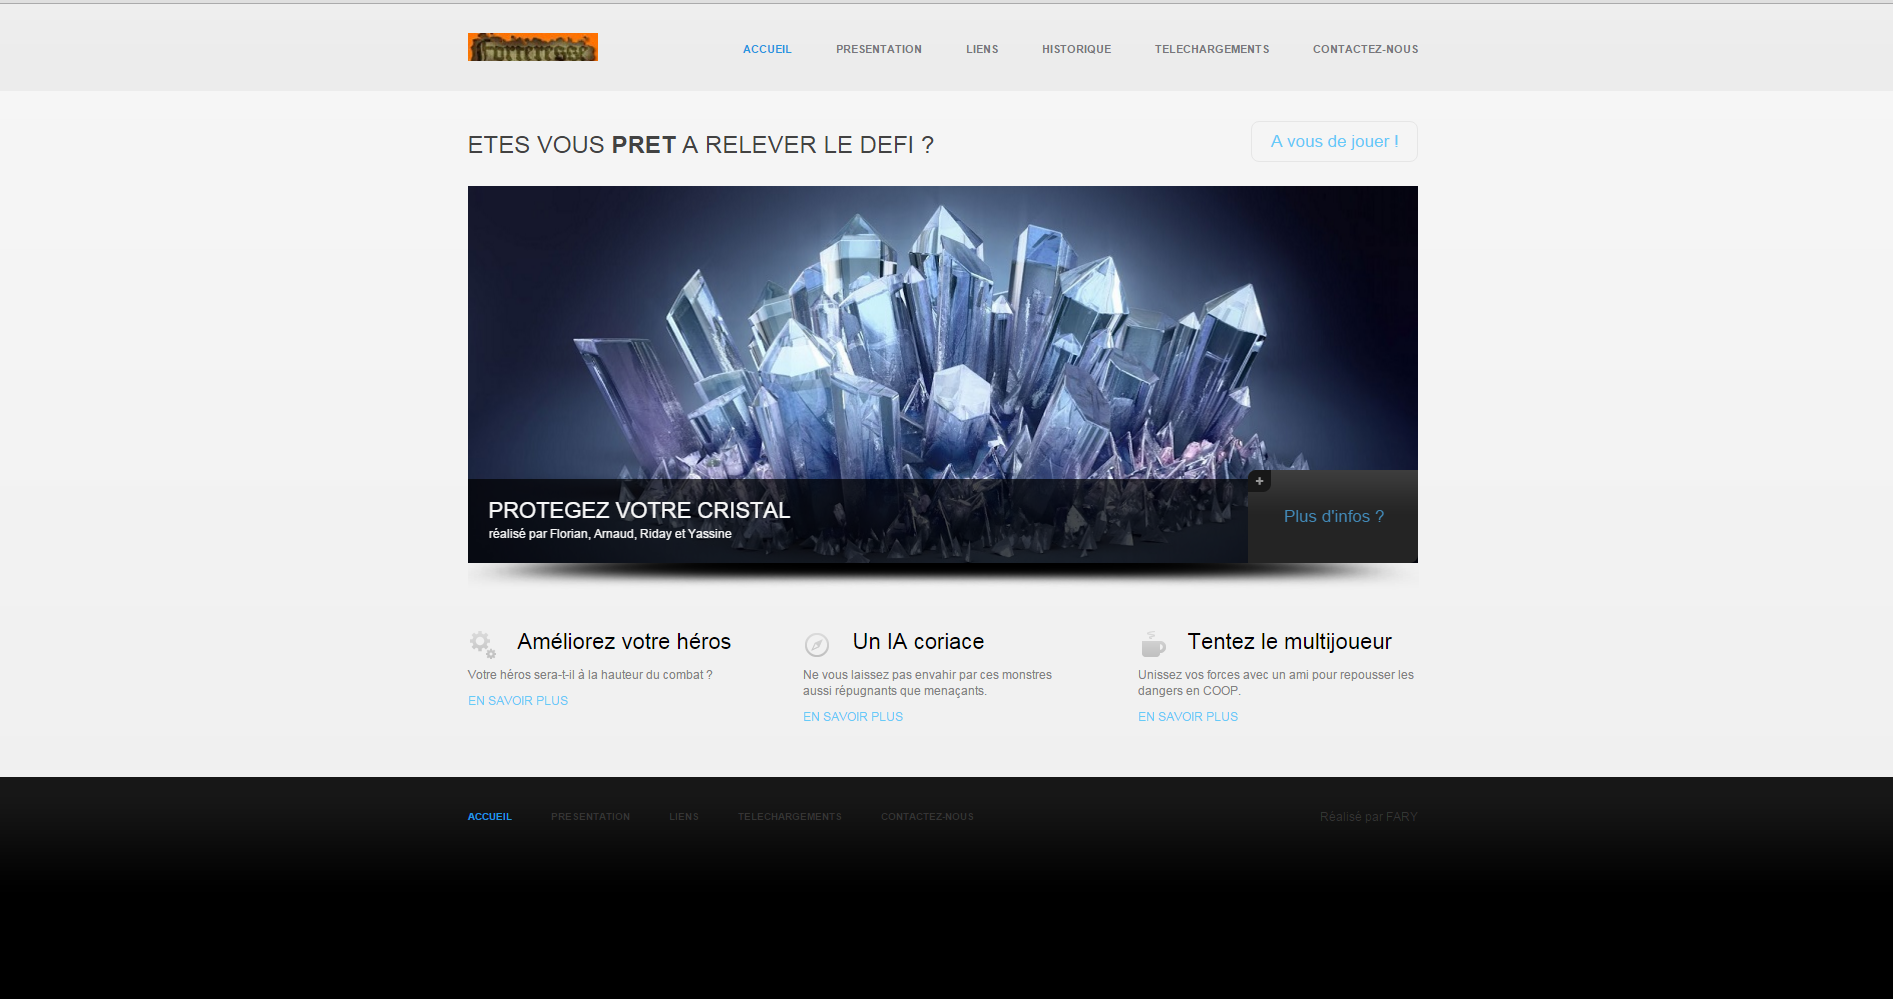
\includegraphics[scale=0.3]{siteprojet.png}}
		\caption*{Page d'accueil du site internet}
	\end{figure}	 
	 
	 Nous avons néanmoins ajouté différents onglets à la page principale tels que la présentation générale du jeu, l’historique de la réalisation du projet que nous remplirons au fur et à mesure, une page pour nous contacter en cas de problèmes ou de questions concernant Forteresse mais également une page où il sera possible de télécharger le jeu en version lite ou normal, ainsi que le cahier des charges. Nous avons également créer un onglet qui vous indique les logiciels utilisés pour réaliser notre jeu ainsi que des liens renvoyant vers le site principal de l’application.

	\subsection{Gameplay}
		\subsubsection{Déplacement}
		Les déplacements ont été le premier élément de gameplay implémenté, puisque c'est un élément indispensable dans tout jeu \'a la troisième personne.
		\par Pour se déplacer, il faut utiliser les touches 'z' pour avancer, 's' pour reculer et on utilise la touche 'q' pour effectuer une rotation sur la gauche et la touche 'd' pour faire une rotation sur la droite. Comme dans la plupart des MMORPG.
		\par Après de nombreux tests, il est apparu que cette façon de se déplacer n'était pas la plus efficace et qu'elle pourrait poser des problèmes notamment pour gérer la visée pour les attaques des personnages. Nous avons donc choisi d'utiliser la souris afin d'effectuer les rotations. Les touches 'q' et 'd' ont donc respectivement été ré-attribué au déplacement latérale gauche et droit.
		\par Le saut s'effectue avec la touche 'espace'. Il ne peut être fait seulement lorsque le personnage est au sol.  
		\subsubsection{Caméra}
		Afin d'améliorer le gameplay au niveau des déplacements, il était important d'avoir un script pour la caméra afin d'avoir une fluidité optimale.
		\par Comme dans la plupart des jeux \'a la troisième personne, la camera suit le personnage de derrière. On contrôle la caméra avec la souris. Il est possible de régler la distance entre la caméra et le personnage à l'aide de la molette de la souris. La caméra gère également les collisions, ce qui lui permet de ne pas passer au travers du sol ou bien de mur.
		\subsubsection{Dégâts}
		La gestion des dégâts et des points de vie, sont deux éléments majeurs du gameplay de notre jeu.
	\begin{figure}[!ht]
		\centerline{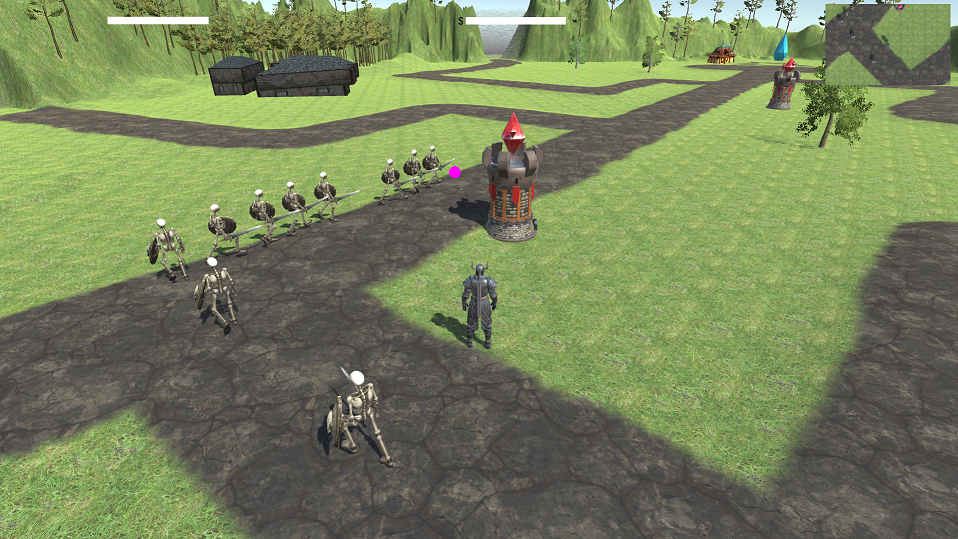
\includegraphics[scale=0.3]{tourattaque.png}}
		\caption*{Image d'une tour qui attaque}
	\end{figure}		

		\par Nous gérons les dégâts de la façon suivante: dans un premier temps un nombre de points de vie est attribué a l'objet (tel qu'un ennemi) et lorsque cet objet entre en collision avec un objet avec un certain tag et un certain nom, un nombre donné de points de vie est retiré à l'objet jusqu'à ce que le nombre de points de vie atteigne 0 et que l'objet soit détruit.
		\subsubsection{La construction}
		La construction d'objets concerne aussi bien la construction de tours que leurs dégâts. En effet pour faire des dégâts, les tours ont besoin de projectiles, il faut donc construire des projectiles lorsque l'ennemi est \'a portée. Pour cela, on clone l'objet qui nous sert de référence, puis on active les scripts nécessaires au bon fonctionnement du projectile sur l'objet cloné.
	\begin{figure}[!ht]	
		\centerline{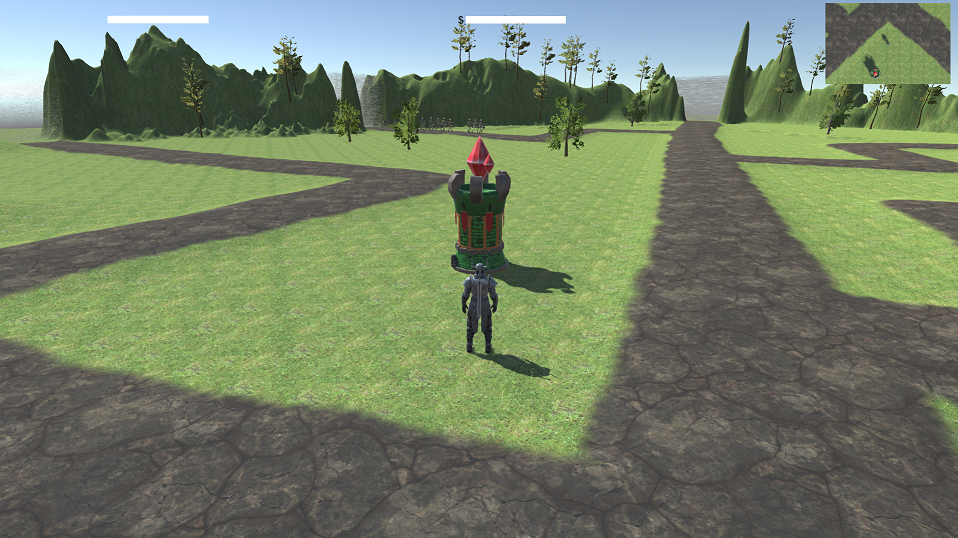
\includegraphics[scale=0.3]{Tour(Clone)projet.png}}	
		\caption*{Image d'une tour en construction}	
	\end{figure}
		
		\par La construction d'une tour utilise le même principe et se déroule en deux étapes. Tout d'abord, la tour va être crée et sera \'a l'état d'image et suivra le personnage, elle sera verte dans les emplacements valides et rouge dans le cas contraire. Une fois la tour positionné \'a l'endroit voulu, un clic gauche permet de la fixer et d'activer ses scripts.
		
		
		\subsubsection{L'apparition des ennemies}
	
		La génération d'ennemie se base sur le même principe que celui de la construction, hormis que les ennemis apparaissent \'a des positions aléatoires autour d'un point, afin d'éviter les problèmes de collision et de blocage entre les différents ennemis. \\
	\begin{figure}[!ht]
		\centerline{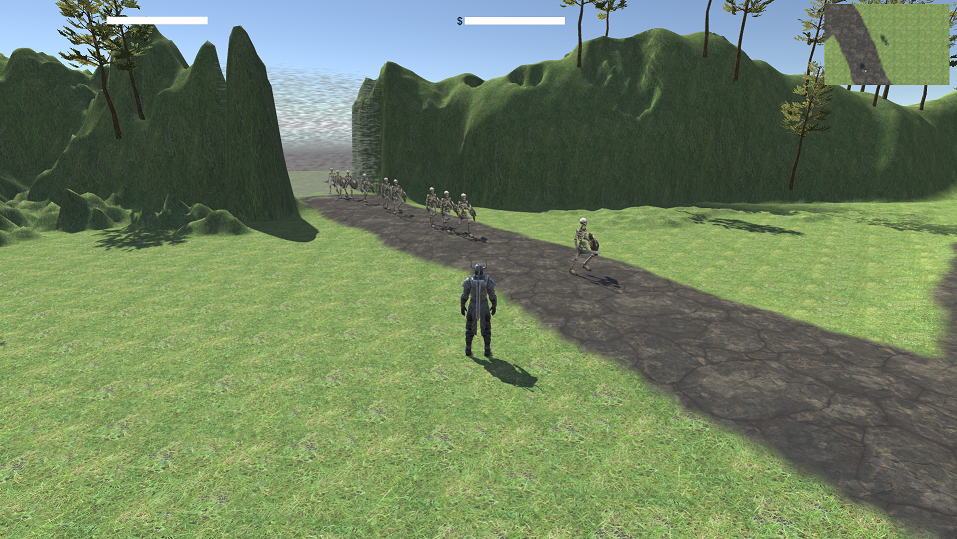
\includegraphics[scale=0.3]{ennemiesprojet.png}}
		\caption*{Apparition d'un vague de squelette}
	\end{figure}

	\subsubsection*{Ce qui est à faire pour la prochaine soutenance}	
	\begin{itemize}
	\item Affectation de points de vie au personnage
	\item Attaque des ennemis
	\item Ajout de tours et d'autre moyen de d\'efense
	\item Ajout de nouveau ennemis 
	\item Système de vague
	\end{itemize}

	\subsection{Animation}
	Pour la partie animation, nous avons du vent qui fait bouger les feuilles des différents arbres présents sur la carte.

\subsubsection*{Ce qui est à faire pour la prochaine soutenance}
\begin{itemize}
\item Animation des personnages
\item Animation des ennemis
\end{itemize}

\section{Planning}
	\begin{tabular}{|c||c|c|c|}
		\hline
		& 1\iere{} soutenance & 2\ieme{} soutenance & 3\ieme{} soutenance \\
		\hline
		Site &  Avancé & Avancé & Terminé \\
		\hline
		3D & Débuté & Avancé & Terminé \\
		\hline
		2D & Débuté & Avancé & Terminé \\
		\hline
		IA & Débuté & Débuté & Terminé\\
		\hline
		Multijoueur & Débuté & Avancé & Terminé\\
		\hline
		Réseau & Débuté & Avancé & Terminé\\
		\hline
		Menu & Avancé & Terminé & Terminé \\
		\hline
		Gameplay & Débuté & Débuté & Terminé\\
		\hline
		Animation & Débuté & Avancé & Terminé\\		
		\hline
		Audio & Non débuté & Débuté & Terminé\\
		\hline		
	\end{tabular}\\
	\newpage
\section{Budget}

Nous sommes des étudiants et ceci est un projet de première année. C'est donc un projet dans le cadre scolaire et à but non lucratif. Ainsi, le budget est de 0\euro{}. Comme prévu aucun achats n'a été nécessaire jusqu'\'a présent pour la réalisation de notre projet. Nous avons utilisé uniquement des logiciels gratuits ou bien fournit gratuitement par l'école. Nous n'avons donc pour le moment aucun dépassement de budget.\\

\centerline{
\includegraphics[scale=0.7]{images.jpg}}

\section{Conclusion}

Les outils à notre disposition pour réaliser le projet étant  nouveaux pour nous, nous avons eu du mal à les utiliser de manière efficace. Nous avons dans la mesure du possible essayé de respecter le planning de la première soutenance. Nous avons des l\'eger retards dans la partie multijoueur, mais avons d\'ebut\'e succinctement la partie audio. De nombreuses tâches restent à réaliser pour la deuxième soutenance. Néanmoins, connaissant mieux les outils mis à notre disposition, nous allons travailler beaucoup plus efficacement et nous espérons, respecter le planning pour la deuxième soutenance. 
\end{document}
